\chapter{\label{sec:implementation}Implementation}

This chapter discusses the implementation details of the system described in the previous chapter. The thesis work aimed to create a proof-of-concept implementation to demonstrate the proposed concepts. 

% - module discovery gossip
% - rating and voting
% - code screenshots
% - LoC + code coverage stats

\section{Overview}

% What is implemented from the framework
% Proof of Concept code
% Can be optimized

This work took a prototyping approach to get to a functioning prototype rapidly and improve from there. All major concepts that were discussed in Chapter 3 were implemented in the proof-of-concept code base. The code was developed alongside the research and served as evaluation of the principles being worked on. 

As the main purpose of the implementation is a proof-of-concept, this code base is not optimized for a production environment. Many different performance and quality optimizations can be done to improve the quality of the implemented product. Examples of these optimizations include:

\begin{itemize}
	\item Implement caching for module database
	\item Remove verbose validations found all over the code
	\item Making the implementation more crash resistant
	\item Better integrate the torrent library by hooking into its event system for notifications 
	\item Improve the user friendliness
\end{itemize}

The final code base can be found publicly on GitHub \footnote{https://github.com/mitchellolsthoorn/ipv8-module-loader}. The programming language that was used for the prototype is Python. Python was chosen because is allows for rapid development and has access to a large collection of existing libraries. Since Python is dynamically typed and allows a lot of flexibility when it comes to security, it also made it easier to implement the proposed concepts in this programming language.The code base consists out of 5000+ lines of code.

During the development of the implementation, several improvements were made and contributed to the overlay library used. This overlay library was only available on GitHub and needed to be used through Git Submodules. By working with the developers of the library we made changes to the library that allowed it to be distributed through the Python Pip package manager. This allows the library to be more easily integrated and used by other developers. The pull requests for these changes can be found on the library's GitHub repository \footnote{https://github.com/Tribler/py-ipv8/pull/402}\footnote{https://github.com/Tribler/py-ipv8/pull/404}\footnote{https://github.com/Tribler/py-ipv8/pull/415}\footnote{https://github.com/Tribler/py-ipv8/pull/448}. Another improvement that was made to the library was a problem discovered in the REpresentational State Transfer (REST) protocol used for communicating with the library backend. This bug made it impossible for HTTP clients that implemented CQRS security to communicate with the library. We proposed a new base endpoint for the REST service that implemented this security protocol that all other endpoints extend from. This rewritten REST service was eventually merged into the main code base of the library. The corresponding pull requests can be found on GitHub \footnote{https://github.com/Tribler/py-ipv8/pull/447}\footnote{https://github.com/Tribler/py-ipv8/pull/458}.

\section{IPv8 - Overlay Library}

IPv8 is the underlying network overlay library used in the implementation. It is responsible for providing \textbf{authenticated} and \textbf{encrypted} communication between different peers (computer nodes) in the system. The framework abstracts the notion of physical addresses (IP addresses) in favor of public keys. This removes the need for applications that use this library to keep track of where different peers in the system are and how to move data between them. IPv8 simplifies the design of distributed overlay systems. 

Some other important aspects of the framework are its focus on:
\begin{itemize}
	\item \textbf{Privacy:} where it is possible to choose if messages should be identifiable to all peers in the network or only to the peers absolutely needed for the network connection (doesn't include the receiver). 
	\item \textbf{No infrastructure dependency:} allowing the network to function on its own run by the peers using the system. This is a very important aspect of the framework as it allows the framework to support itself, without needing external financing for server capacity.
	\item \textbf{NAT traversal:} making it possible to operate the network without static servers needed for overcoming the NAT issues that most peer-to-peer networks face.
	\item \textbf{Trust:} one of the most important aspects of peer-to-peer systems, as it is needed to mitigate free-riding issues in the network. In IPv8 trust is gained by recording a patterns of previous actions and storing these on a blockchain structure called TrustChain.
\end{itemize}

The last main aspect of the framework is \textbf{extensibility}. IPv8 makes use of a concept called overlays. Where a virtual network is created in the system related to one specific application domain or topic where different peers can subscribe to. This is a very powerful mechanism to allow extendability and modularization of an specific application. This makes it possible for user applications to be run alongside the FBase framework.

\section{Framework Structure}

This section will go over the major components of the code and explain the folder structure used in the implementation. The root directory of the project consists out of two folders:
\begin{itemize}
	\item \textbf{module\_loader:} The module loader directory serves as a python package for the entire code base of the prototype. All the major components of the framework are located in this directory.
	\item \textbf{twisted/plugins:} The twisted plugins directory is a mandatory location for the storage of the framework main application files. This requirement comes from the library Twisted which IPv8 is built on. This library provides pseudo multi-threading by implementing an event based scheduler.
\end{itemize}

Inside the module loader python package the following structure is used:

\begin{itemize}
	\item \textbf{CLI:} The CLI package contains all classes and logic related to the command-line user interface of the framework. This is the primary way to manage the network.
	\item \textbf{community:} The community package contains the overlay code. This includes the majority of all logic related to the FBase functionality.
	\item \textbf{event:} The event package contains all classes and functionality related to the main event bus of the FBase framework.
	\item \textbf{REST:} The REST package contains all REST endpoints needed to communicate with the FBase backend from other applications and services. This interface also allows user applications to communicate with their frontend
	\item \textbf{web:} The web directory contains the web frontend for the FBase framework. This is an alternative way for managing the framework next to the CLI.
\end{itemize}

\section{Community}

The community class is the main overlay class that manages all parts of the FBase module network. This class acts as the controller for all inputs and outputs of the system.

Figure \ref{fig:community-code} and \ref{fig:community-code-imports} show snippets of the community code base as the central part of the application logic.

\begin{figure}[h!]
	\centering
	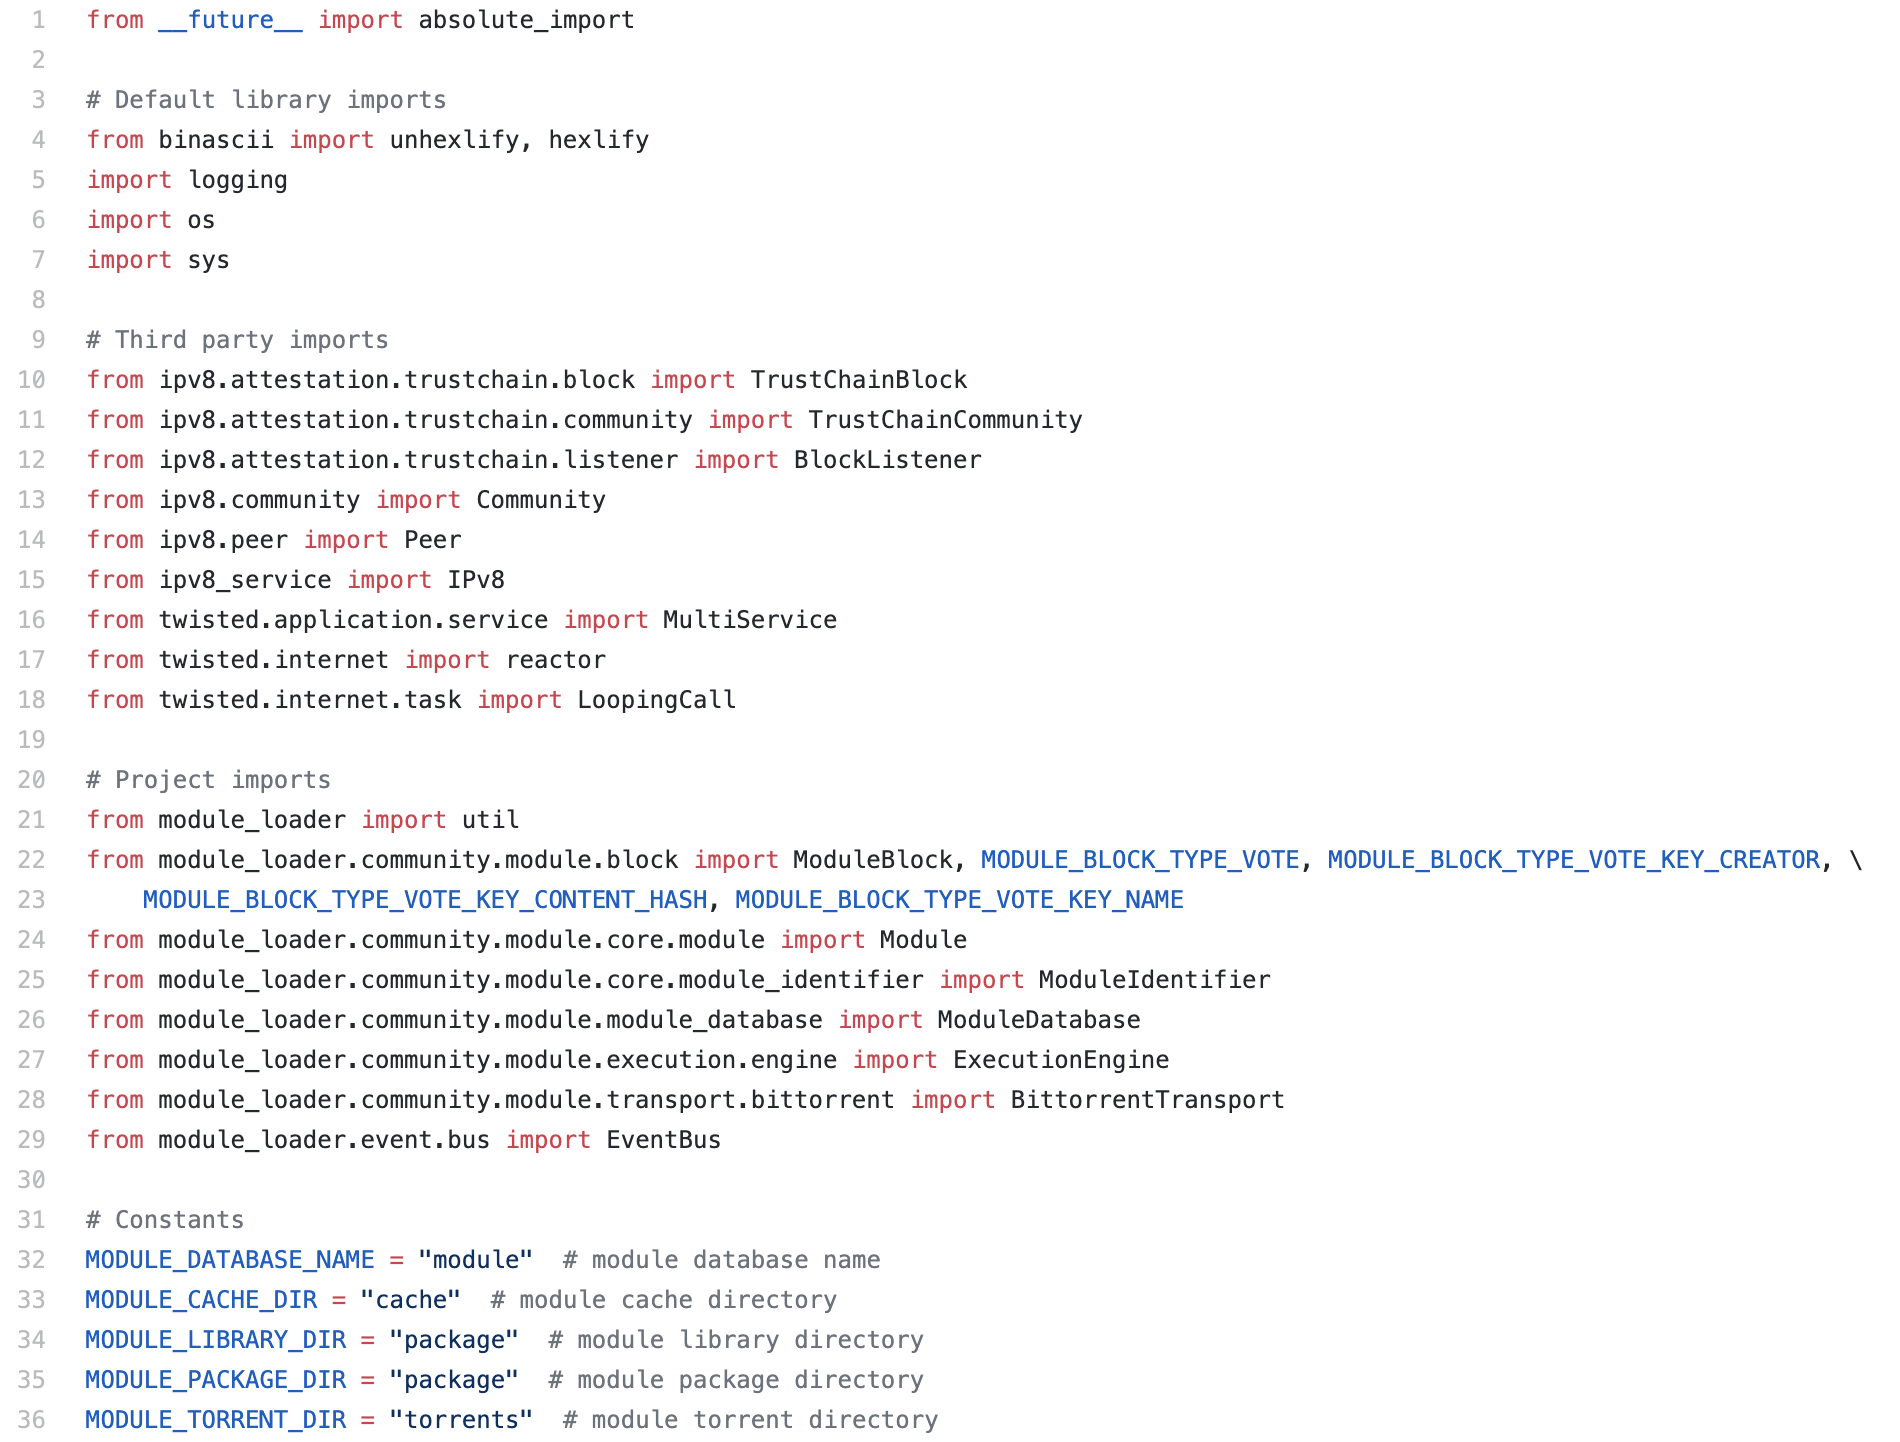
\includegraphics[width=\textwidth]{images/code-community-imports.png}
	\caption{\label{fig:community-code-imports}}
\end{figure}

\begin{figure}[h!]
	\centering
	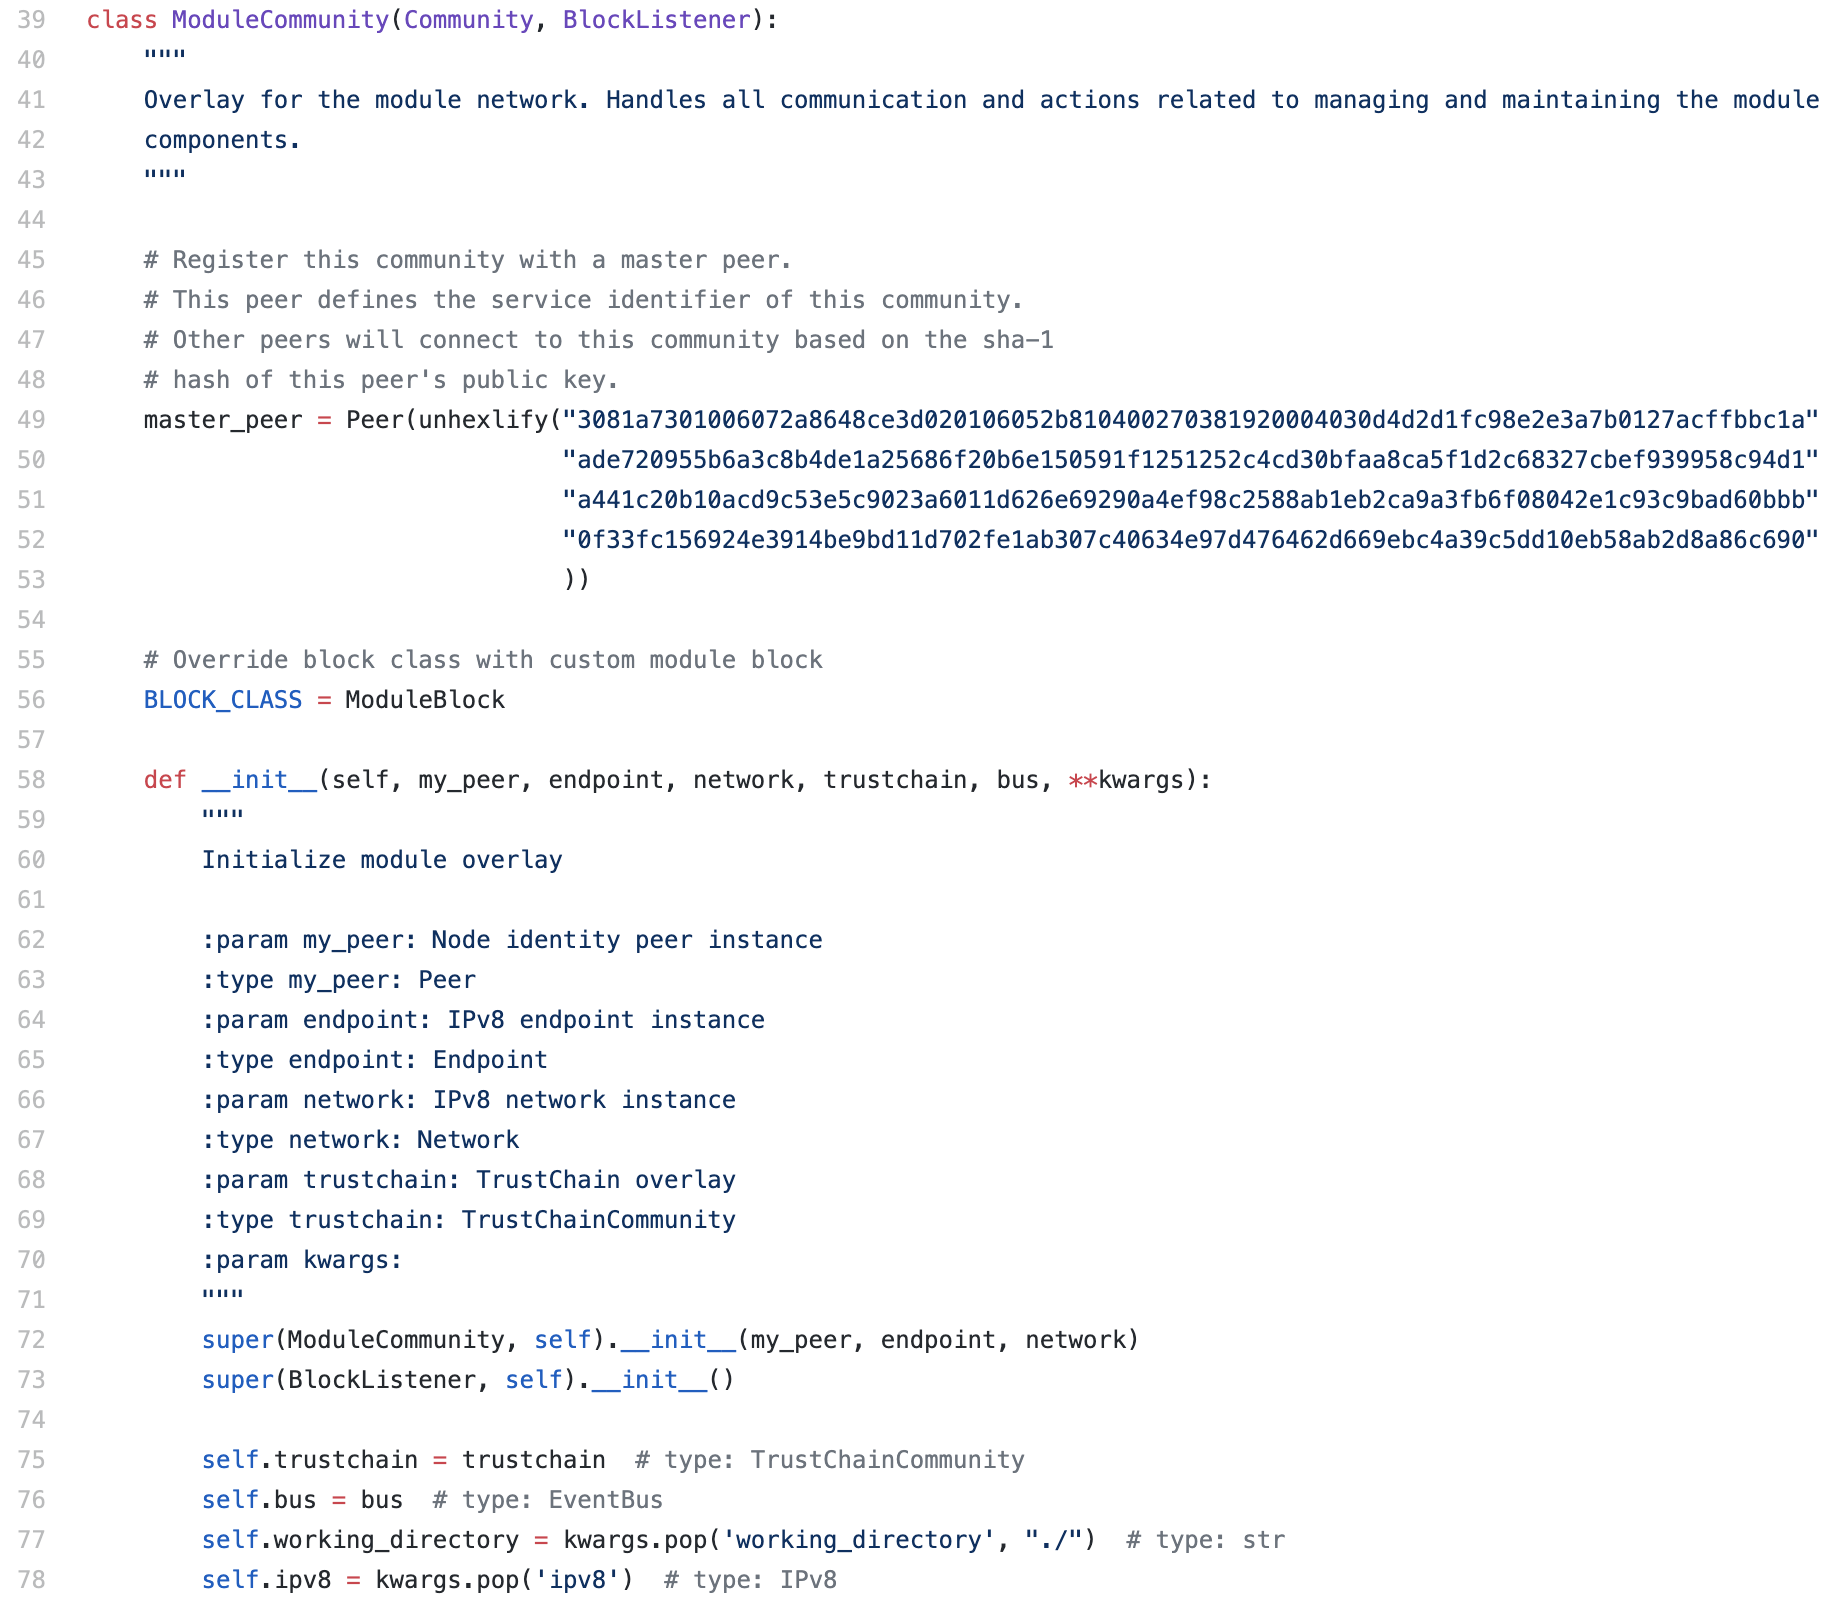
\includegraphics[width=\textwidth]{images/code-community-class.png}
	\caption{\label{fig:community-code}}
\end{figure}

\section{Event Bus}

The event bus that is implemented in the FBase prototype is built according to a PubSub design pattern. In this design pattern, modules can register themselves to receive messages when an event has been fired with a certain event type. These registered modules, also called subscribers, are store in an array in memory. They only receive a call when that event is fired. Modules that publish event, called publisher, call the event bus with the message and the type of the message.

In the prototype the event bus is implemented in code. For production use, however, it might be a good improvement to run the event bus as a separate process to speed up the performance when many event are being fired at a time. It would also allow multiple processes to be used to handle the actions performed by the subscribers. 

\section{Interface}

There are two interfaces through which the FBase framework can be managed. Originally only the CLI interface was used. Later in development the web interface was added to allow the framework to be controlled from any platform the framework runs. This decision was made since the framework itself could be run cross-platform, but it could only be controlled from platforms that support a CLI.

\subsection{CLI}
The CLI interface operates through a command line menu interface. This menu allows the user of the framework to run sets of actions. The general actions are

\begin{itemize}
	\item \textbf{List all modules:} This action provides a list with context actions. Each of these context actions are performed on the module that is selected by the user.
	\item \textbf{Create test module:} Create an empty test module that can be used for testing the distribution of modules through the network.
	\item \textbf{Create module:} Create a module from a module definition that exists on the file system. The module should already be created. This action only processes the module and prepares the metadata for publishing it on the network.
\end{itemize}

The context menu for each module shows information about the module. It includes the name of the module, the description, the identifier and the number of votes in the network for the module. Next to this information there are also context actions that are displayed and can be called. The context actions include:

\begin{itemize}
	\item \textbf{Vote:} This context actions instructs the backend of the framework to sign the corresponding vote block that will be created. This vote block will then be distributed through the network.
	\item \textbf{Download:} The download context action retrieves the identifier of the module and starts the download of the module through the transport engine.
	\item \textbf{Run:} The run context action loads the module package namespace into the Python path of the framework. Afterwards it start the application based on the instructions provided in the module.
\end{itemize}

Figure \ref{fig:cli-interface} shows a screenshot of the CLI interface showing the list of discovered modules. Figure \ref{fig:cli-code} shows a snippet of the code that is responsible for the CLI interface.

\begin{figure}[h!]
	\centering
	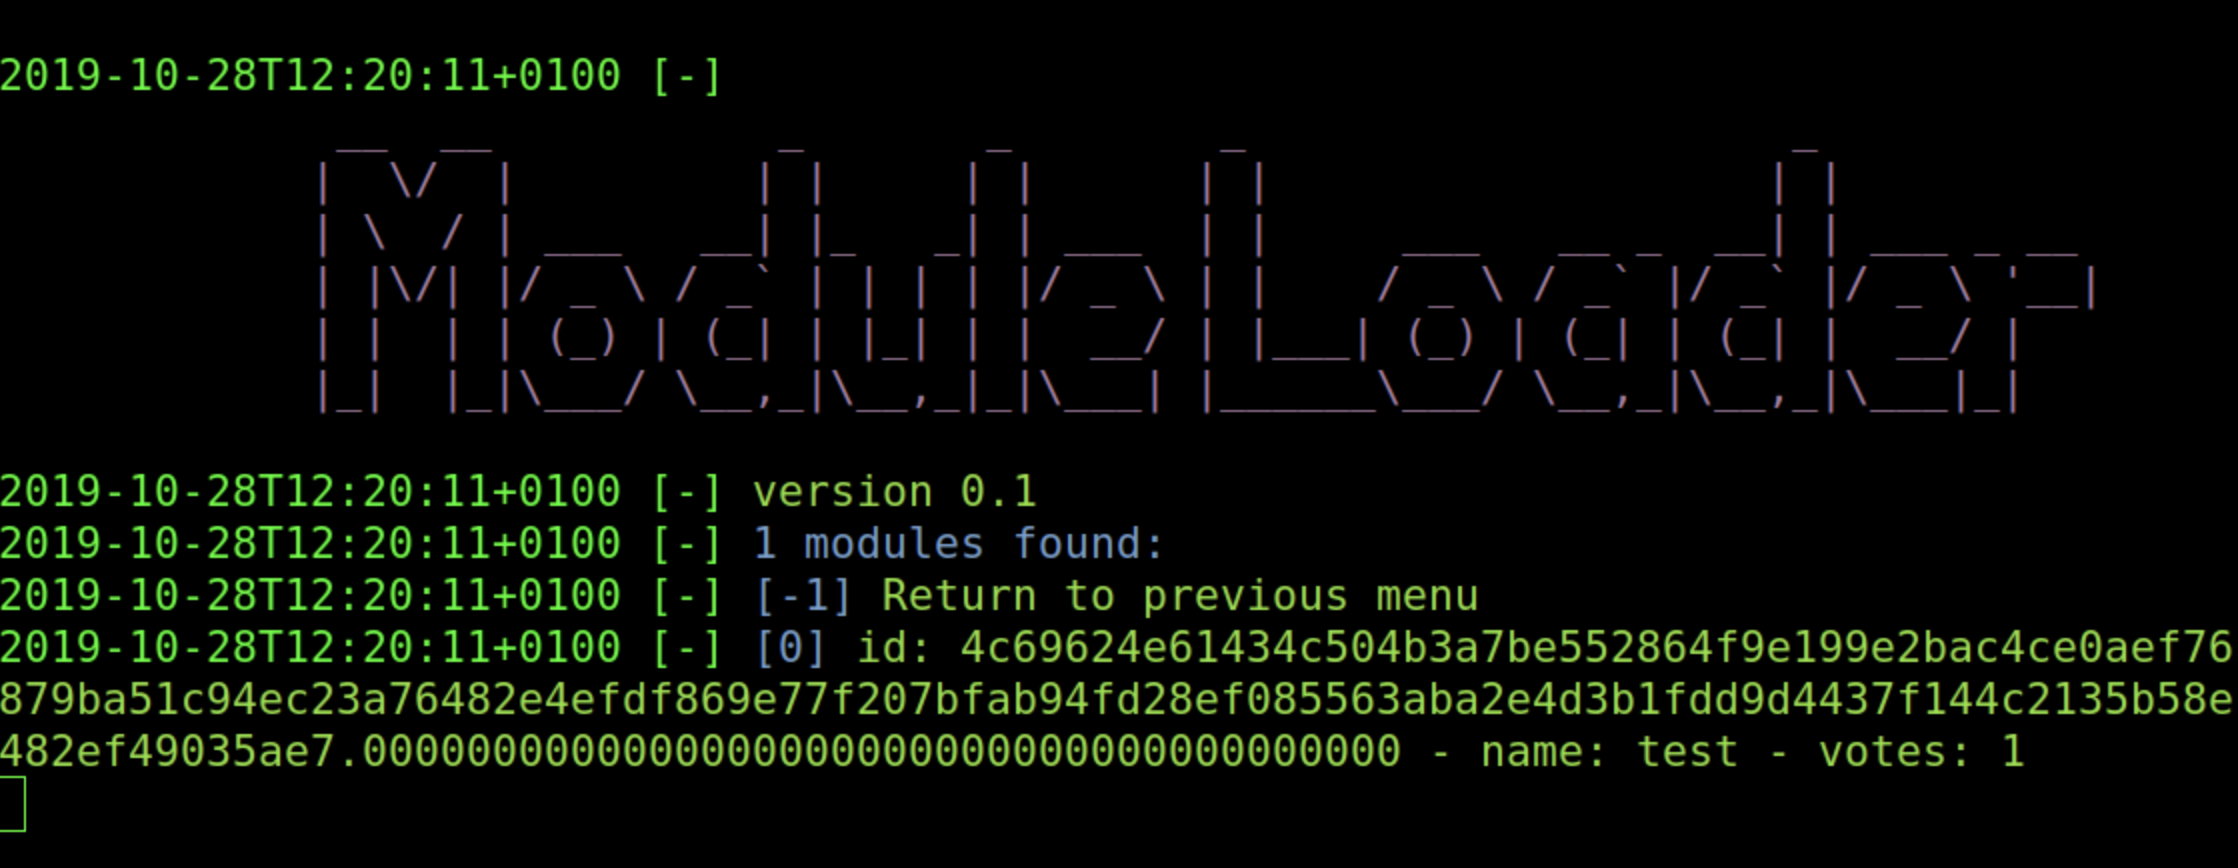
\includegraphics[width=\textwidth]{images/cli-interface.png}
	\caption{\label{fig:cli-interface}}
\end{figure}

\begin{figure}[h!]
	\centering
	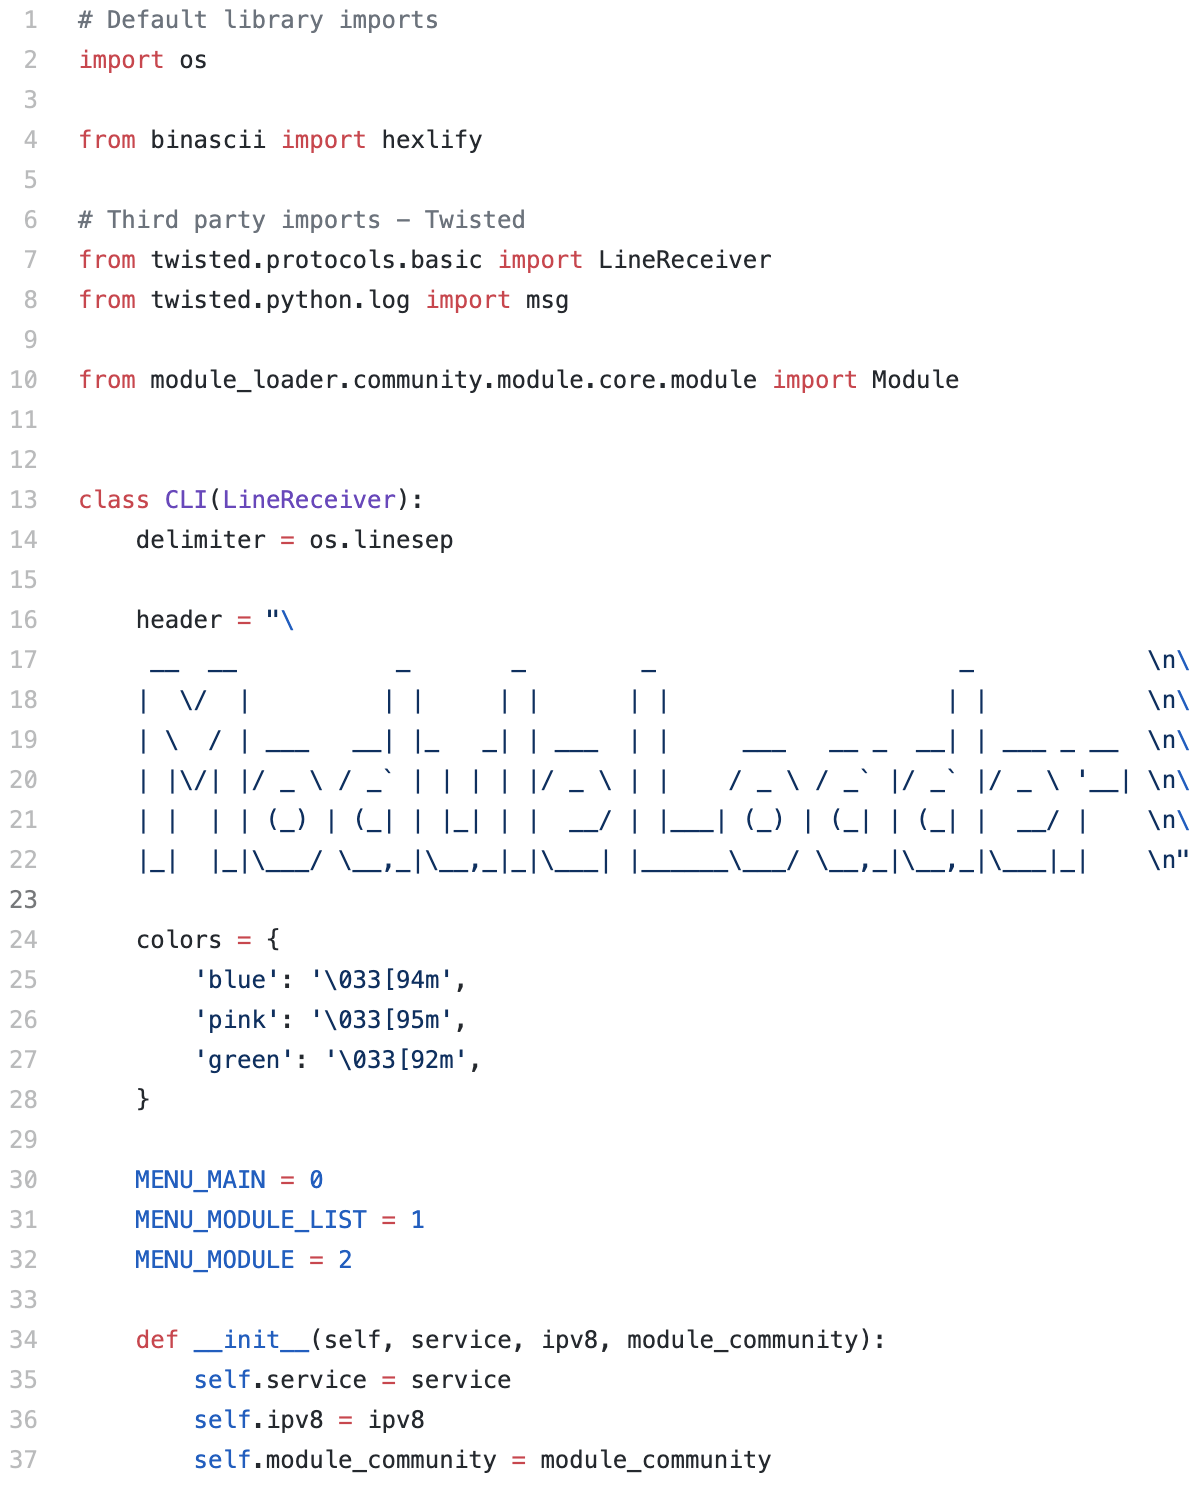
\includegraphics[width=\textwidth]{images/code-cli.png}
	\caption{\label{fig:cli-code}}
\end{figure}

\subsection{Web Interface}

The web interface is a website built with HTML, CSS, and JavaScript that runs as a standalone service that communicates with the FBase backend through the REST API. This interface allows to view all discovered modules, download them and run them. This interface does not allow module to be created.

\section{REST Endpoints}

The FBase framework provides several REST endpoints on its API for the web interface to operate. These API endpoints can also be used by other applications to perform actions on the overlay network.

\begin{itemize}
	\item \textbf{Catalog:} The catalog endpoint is responsible for all actions related to the discovered modules on the network. This endpoint is mostly used for retrieving information about the modules available.
	\item \textbf{Downloads:} The downloads endpoint is responsible for managing modules that need to be downloaded or are already downloaded. Its action include the downloading of modules, the deletion of modules from the host, and to retrieve the status about the downloaded modules.
	\item \textbf{Library:} The library endpoint is used to manage all modules that are currently being used by user applications on the framework.
	\item \textbf{Run:} The run endpoint provides actions to load and run the module that is specified.
	\item \textbf{Votes:} The votes endpoint is responsible for all action related to voting and managing votes that have been performed.
\end{itemize}

Figure \ref{fig:rest-cors} shows a snippet of the code that is responsible for performing the CORS security protocol.

\begin{figure}[h!]
	\centering
	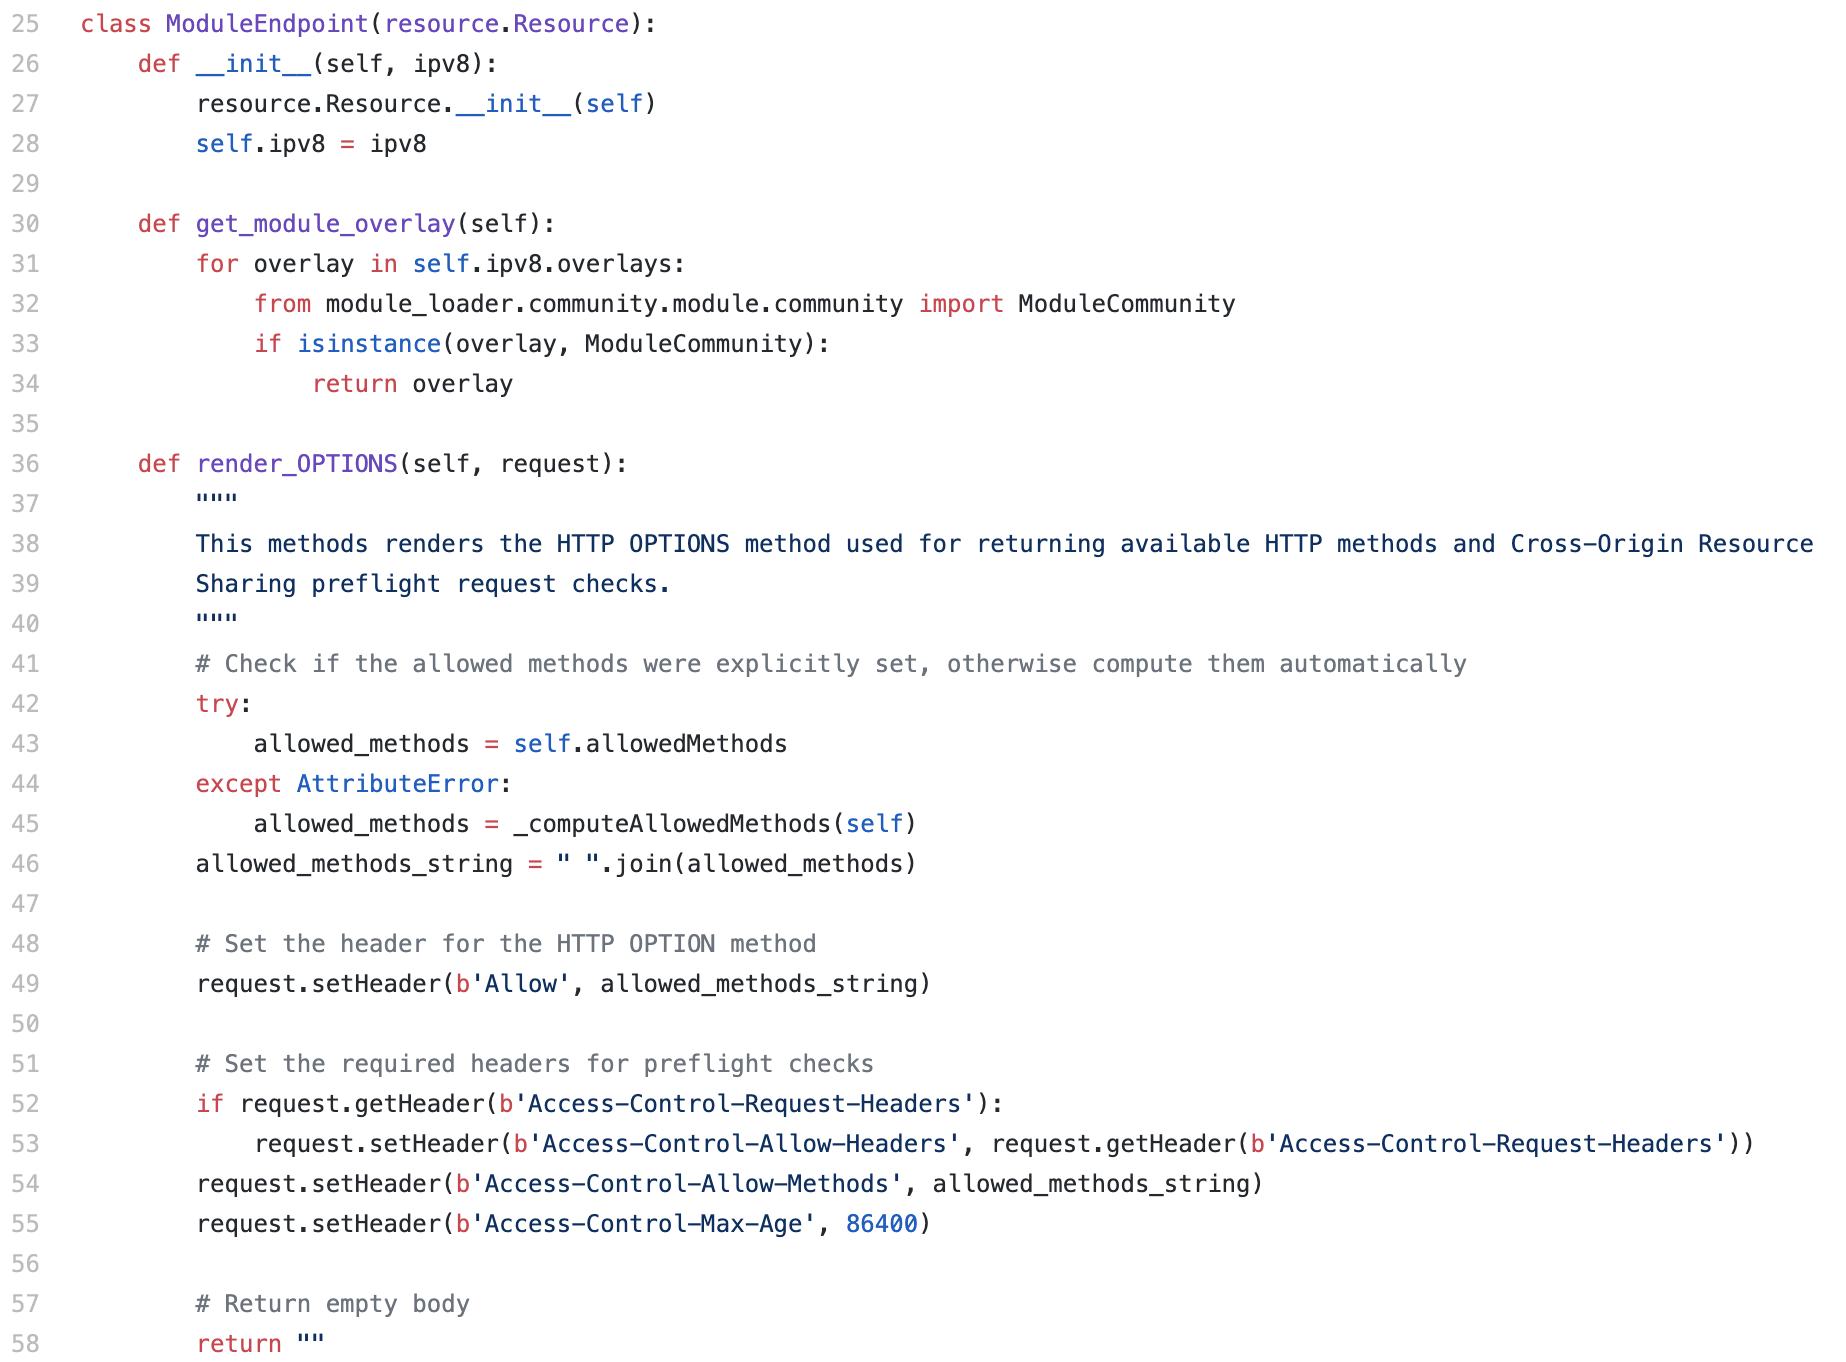
\includegraphics[width=\textwidth]{images/code-rest-cors.png}
	\caption{\label{fig:rest-cors}}
\end{figure}



\section{Module Structure}

This section will expand on the structure used for modules in the framework. Each module in the framework has to be a valid Python package. This is done to make it easier to import the module on runtime. This requires the module to have an \_\_init\_\_.py file in its root directory. Besides this each module must also have a manifest.json file. This manifest file specifies the type of module and its information. Without this file the module will not be detected and can not be run.

This manifest file contains a JSON dictionary. This dictionary contains key value pairs for all the information required.

\begin{itemize}
	\item \textbf{Name:} Specifies the name of the module used for displaying in the user interface
	\item \textbf{Description:} Specifies the description of the module used for determining if a user wants to download and use the module 
	\item \textbf{Version:} Specifies the version of the module to determine if tthis is the most current version of the module
	\item \textbf{Type:} Specifies the type of the module, determining how it needs to be run and what kind of modules can require it.
	\item \textbf{Dependencies:} Specifies the other modules this module relies on.
\end{itemize}


\section{Module Distribution}
 The module distribution method was chosen based on the ability to setup an integrated content distribution network that would work efficiently and scale. Since this is not the first time this is done and there already exist excellent solutions out there that could accomplish this.

\subsubsection{\textbf{Web protocols}}

Web protocols like HyperText Transfer Protocol (HTTP) and its secure variant HTTPS are a very common transfer protocol in the current day internet. It is used by all major Linux distribution to distribute the system packages, by websites for downloading content and watching videos. This protocol supports file transfer resumes, encryption. It, However, doesn't scale well when the same content has to be uploaded to multiple users and doesn't natively provide content verification.

\subsubsection{\textbf{BitTorrent}}

BitTorrent is the protocol used by all bittorrent clients. It provides encryption, content verification, file transfer resumes, and scales very well when large amounts of the same contents has to be distributed thanks to its mesh architecture. That is why this protocol was selected as the basis of the module distribution of this work.

BitTorrent also has the advantage of having a Distributed Hash Table (DHT). This DHT stores all information about who has a copy of the content and the meta data needed to download it in a distributed fashion. This removes the need for FBase to implement its own mechanism for this.

BitTorrent is the protocol used in the proof-of-concept.

\section{Discovery and Voting}

When a suitable transfer protocol is chosen, the next step was to make it possible for modules to be discoverable by all nodes in the system. Since we were already building our framework on top of the IPv8 peer-to-peer communication library. We decided it would be a good fit to use this to accomplish our goal, since it was very suited for bulk small size data gossiping. So this became out chosen method of module discovery.

Since IPv8 also provides a block-chain storage back-end it was an perfect opportunity to also implement voting on the IPv8 library.

When a vote is done a block is created to represent this vote. This block is then store on a blockchain. The reason we store the votes on the blockchain is to make votes irrefutable. Voting is unidirectional. Permission should not be needed from the other side. This is represented in the blockchain by only one party signing the vote. Storing votes on the blockchain also prevents malicious use of votes to promote ones one module.

\section{Blockchain}

The FBase prototype is built on the
TrustChain ledger introduced by Otte et al. We identified
two advantages of TrustChain over other pairwise distributed
ledgers like R3 Corda and Nano. First, TrustChain focuses
on fraud detection instead of prevention and as a result does
not require network-wide consensus. This makes TrustChain
a lightweight and simple data structure. Second, TrustChain is
already used as transaction fabric within a self-sovereign, decentralized identity system, described in the work of Stokkink
et al. Availability of a self-sovereign identity system
aligns with our requirement for strong, long-lived identities.